\documentclass[tikz,border=8pt]{standalone}
\usetikzlibrary{arrows.meta,positioning,shapes.geometric}
\begin{document}
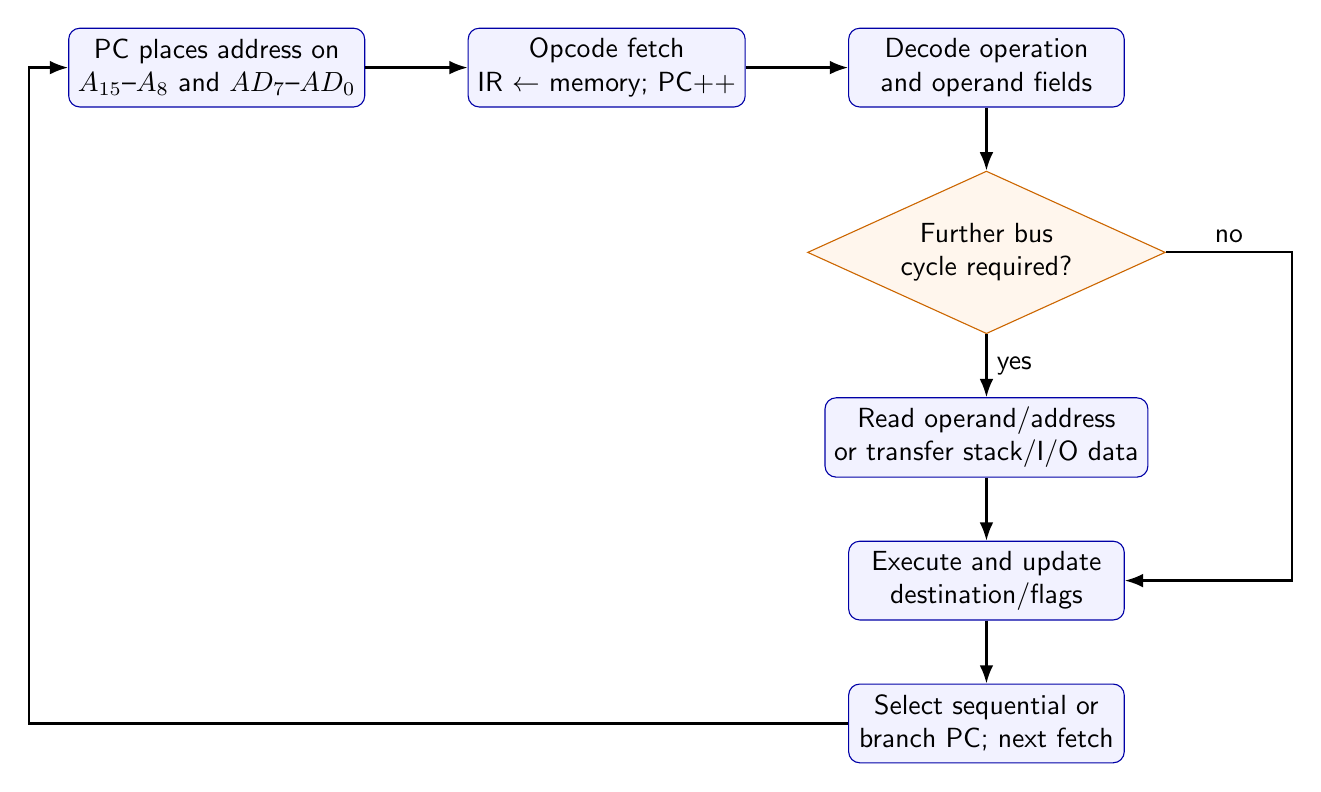
\begin{tikzpicture}[font=\sffamily,>=Latex,node distance=8mm and 13mm,
proc/.style={draw=blue!65!black,rounded corners,fill=blue!5,minimum width=35mm,minimum height=10mm,align=center},
decision/.style={diamond,draw=orange!80!black,fill=orange!7,aspect=2.2,align=center},
arr/.style={->,thick}]
\node[proc] (pc) {PC places address on\\$A_{15}$--$A_8$ and $AD_7$--$AD_0$};
\node[proc,right=of pc] (fetch) {Opcode fetch\\IR $\leftarrow$ memory; PC$++$};
\node[proc,right=of fetch] (decode) {Decode operation\\and operand fields};
\node[decision,below=of decode] (more) {Further bus\\cycle required?};
\node[proc,below=of more] (operand) {Read operand/address\\or transfer stack/I/O data};
\node[proc,below=of operand] (execute) {Execute and update\\destination/flags};
\node[proc,below=of execute] (next) {Select sequential or\\branch PC; next fetch};
\draw[arr] (pc)--(fetch); \draw[arr] (fetch)--(decode); \draw[arr] (decode)--(more);
\draw[arr] (more)--node[right]{yes}(operand); \draw[arr] (operand)--(execute);
\draw[arr] (more.east)--node[above]{no}++(16mm,0)|-(execute.east);
\draw[arr] (execute)--(next); \draw[arr] (next.west)-|([xshift=-5mm]pc.west)--(pc.west);
\end{tikzpicture}
\end{document}
